% ==============================================================================
% Chapter 4: Methodology
% ==============================================================================

\chapter{Methodology}
\label{ch:methodology}

% ------------------------------------------------------------------------------
% 4.1 Overview
% ------------------------------------------------------------------------------
\section{Overview}
\label{sec:meth-overview}

This chapter presents the detailed methodology employed to investigate the research questions posed in this thesis. The methodology is designed to enable a rigorous and fair comparison between the baseline SPAM-XAI pipeline and the proposed enhanced pipeline that substitutes autoencoders for PCA and XGBoost for MLP while preserving SMOTE for class balancing and LIME for explainability.

The chapter is organized as follows. Section~\ref{sec:research-design} describes the overall research design and experimental framework. Section~\ref{sec:datasets} presents the datasets used for evaluation, including their characteristics and class distributions. Section~\ref{sec:preprocessing} details the data preprocessing pipeline applied to both approaches. Section~\ref{sec:imbalance-handling} describes the SMOTE configuration for handling class imbalance. Section~\ref{sec:pipeline-configs} presents the detailed configurations of both the baseline and proposed pipelines, including architecture specifications and hyperparameter settings. Section~\ref{sec:implementation} describes the implementation environment, including hardware, software, and libraries used. Section~\ref{sec:eval-metrics} defines the evaluation metrics employed to assess classification performance. Section~\ref{sec:xai-methodology} outlines the methodology for generating and evaluating LIME explanations. Finally, Section~\ref{sec:meth-summary} summarizes the methodological approach.

% ------------------------------------------------------------------------------
% 4.2 Research Design
% ------------------------------------------------------------------------------
\section{Research Design}
\label{sec:research-design}

This research adopts an empirical, experimental methodology following established practices in software defect prediction research \parencite{hall2012systematic}. The design enables controlled comparison between pipeline configurations while isolating the effects of individual component substitutions.

\subsection{Experimental Framework}
\label{subsec:exp-framework}

The experimental framework is structured as a comparative study between two software defect prediction pipelines:

\begin{enumerate}
    \item \textbf{Pipeline A (Baseline SPAM-XAI):} Implements the established SPAM-XAI approach combining SMOTE for class balancing, PCA for dimensionality reduction, MLP for classification, and LIME for explainability.
    
    \item \textbf{Pipeline B (Proposed):} Modifies the baseline by substituting a shallow autoencoder for PCA and XGBoost for MLP, while retaining SMOTE and LIME to enable direct comparison of the dimensionality reduction and classification components.
\end{enumerate}

Figure~\ref{fig:pipeline-comparison} illustrates the architectural differences between the two pipelines.

\begin{figure}[htbp]
    \centering
    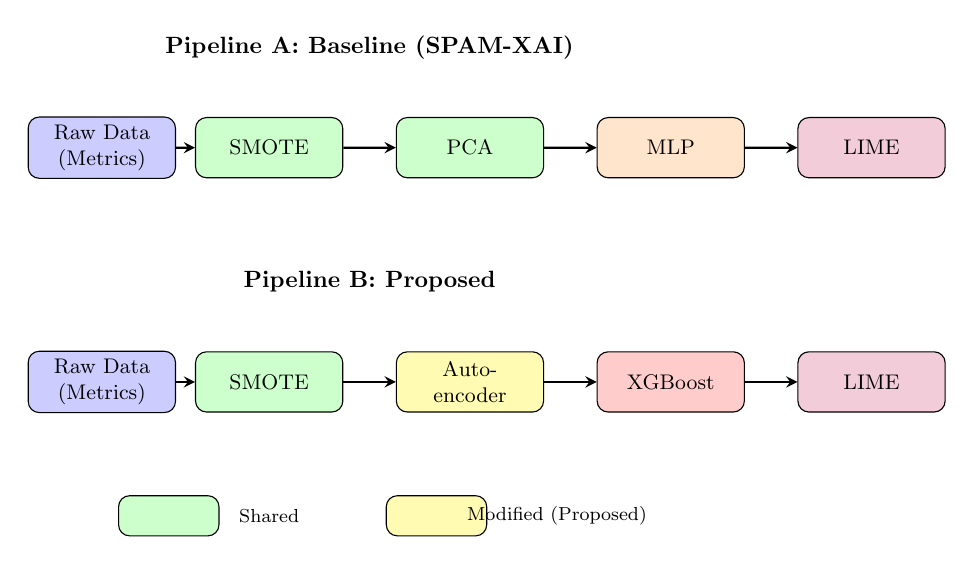
\begin{tikzpicture}[
        scale=0.85,
        transform shape,
        box/.style={draw, rounded corners, minimum width=2.2cm, minimum height=0.9cm, align=center, font=\small},
        data/.style={box, fill=blue!20},
        process/.style={box, fill=green!20},
        model/.style={box, fill=orange!20},
        xai/.style={box, fill=purple!20},
        arr/.style={->, thick, >=stealth}
    ]
        % Pipeline A - Baseline
        \node[font=\bfseries] at (0, 4.5) {Pipeline A: Baseline (SPAM-XAI)};
        
        \node[data] (dataA) at (-4, 3) {Raw Data\\(Metrics)};
        \node[process] (smoteA) at (-1.5, 3) {SMOTE};
        \node[process] (pcaA) at (1.5, 3) {PCA};
        \node[model] (mlpA) at (4.5, 3) {MLP};
        \node[xai] (limeA) at (7.5, 3) {LIME};
        
        \draw[arr] (dataA) -- (smoteA);
        \draw[arr] (smoteA) -- (pcaA);
        \draw[arr] (pcaA) -- (mlpA);
        \draw[arr] (mlpA) -- (limeA);
        
        % Pipeline B - Proposed
        \node[font=\bfseries] at (0, 1) {Pipeline B: Proposed};
        
        \node[data] (dataB) at (-4, -0.5) {Raw Data\\(Metrics)};
        \node[process] (smoteB) at (-1.5, -0.5) {SMOTE};
        \node[process, fill=yellow!30] (aeB) at (1.5, -0.5) {Auto-\\encoder};
        \node[model, fill=red!20] (xgbB) at (4.5, -0.5) {XGBoost};
        \node[xai] (limeB) at (7.5, -0.5) {LIME};
        
        \draw[arr] (dataB) -- (smoteB);
        \draw[arr] (smoteB) -- (aeB);
        \draw[arr] (aeB) -- (xgbB);
        \draw[arr] (xgbB) -- (limeB);
        
        % Legend
        \node[process, minimum width=1.5cm, minimum height=0.6cm] at (-3, -2.5) {};
        \node[font=\footnotesize] at (-1.5, -2.5) {Shared};
        \node[process, fill=yellow!30, minimum width=1.5cm, minimum height=0.6cm] at (1, -2.5) {};
        \node[font=\footnotesize] at (2.8, -2.5) {Modified (Proposed)};
    \end{tikzpicture}
    \caption{Comparison of Pipeline A (baseline SPAM-XAI) and Pipeline B (proposed). Yellow-highlighted components indicate modifications in the proposed pipeline: autoencoder replaces PCA, and XGBoost replaces MLP.}
    \label{fig:pipeline-comparison}
\end{figure}

\subsection{Comparative Analysis Approach}
\label{subsec:comparative-approach}

The comparative analysis is designed to answer the research questions by isolating the effects of component substitutions:

\begin{itemize}
    \item \textbf{Controlled Variables:} Both pipelines use identical datasets, preprocessing steps, train-test splits, SMOTE configurations, and LIME settings. This ensures that observed performance differences can be attributed to the dimensionality reduction and classification components.
    
    \item \textbf{Independent Variables:} The dimensionality reduction method (PCA vs. autoencoder) and classifier (MLP vs. XGBoost) are the primary independent variables.
    
    \item \textbf{Dependent Variables:} Classification performance metrics (Precision, Recall, F1-score, AUC-ROC, MCC) and explanation characteristics serve as dependent variables.
\end{itemize}

% ------------------------------------------------------------------------------
% 4.3 Datasets
% ------------------------------------------------------------------------------
\section{Datasets}
\label{sec:datasets}

The experiments utilize datasets from the NASA PROMISE repository, a widely-used benchmark collection for software defect prediction research \parencite{menzies2007promise}. The PROMISE repository provides standardized, publicly available datasets that enable reproducible research and meaningful comparison with prior work.

\subsection{NASA PROMISE Repository}
\label{subsec:promise-repo}

The NASA PROMISE (PRedictOr Models In Software Engineering) repository was established to address reproducibility concerns in software engineering research by providing curated datasets with consistent formats and documentation. The datasets used in this study are obtained from the tera-PROMISE repository \parencite{menzies2007promise}, accessible at \url{https://openscience.us/repo/defect/mccabehalsted/}. This repository provides cleaned versions of the original NASA MDP datasets and has been widely used in defect prediction studies \parencite{hall2012systematic}. Data quality considerations follow the recommendations of \textcite{shepperd2013data}, who documented issues in earlier versions of these datasets.

The datasets contain static code metrics extracted from NASA software projects, including complexity measures (cyclomatic complexity, Halstead metrics), size metrics (lines of code, number of operators/operands), and module-level attributes. Each module is labeled as either defective (containing at least one post-release defect) or clean.

\subsection{Dataset Characteristics}
\label{subsec:dataset-chars}

Three datasets are selected for this study, chosen to enable comparison with prior SPAM-XAI research and to represent varying project characteristics and imbalance levels:

\textbf{CM1.} The CM1 dataset originates from a NASA spacecraft instrument project written in C. It contains 498 modules characterized by 21 static code metrics. The defect rate is approximately 10\%, representing moderate class imbalance.

\textbf{PC1.} The PC1 dataset is derived from flight software for an Earth-orbiting satellite, also written in C. It comprises 1,109 modules with 21 metrics. The defect rate is approximately 7\%, exhibiting higher imbalance than CM1.

\textbf{PC2.} The PC2 dataset comes from a dynamic simulator for attitude control systems. It is the largest dataset with 5,589 modules and 36 metrics. The defect rate is approximately 1\%, representing severe class imbalance.

\subsection{Dataset Statistics and Class Distribution}
\label{subsec:dataset-stats}

Table~\ref{tab:dataset-stats} summarizes the key statistics of the three datasets, including the number of modules, features, and class distribution.

\begin{table}[htbp]
\centering
\caption{Summary statistics of the NASA PROMISE datasets used in this study}
\label{tab:dataset-stats}
\begin{tabular}{@{}lccccc@{}}
\toprule
\textbf{Dataset} & \textbf{Modules} & \textbf{Features} & \textbf{Defective} & \textbf{Clean} & \textbf{Defect Rate} \\
\midrule
CM1 & 498 & 21 & 49 & 449 & 9.84\% \\
PC1 & 1,109 & 21 & 77 & 1,032 & 6.94\% \\
PC2 & 5,589 & 36 & 23 & 5,566 & 0.41\% \\
\bottomrule
\end{tabular}
\end{table}

The metrics included in these datasets fall into several categories:

\begin{itemize}
    \item \textbf{Size metrics:} Lines of code (LOC), number of blank lines, number of comments.
    \item \textbf{Halstead metrics:} Program length, vocabulary, volume, difficulty, effort, time to program, and delivered bugs estimate.
    \item \textbf{McCabe complexity:} Cyclomatic complexity, essential complexity, design complexity.
    \item \textbf{Miscellaneous:} Number of unique operators, number of unique operands, total operators, total operands.
\end{itemize}

% ------------------------------------------------------------------------------
% 4.4 Data Preprocessing Pipeline
% ------------------------------------------------------------------------------
\section{Data Preprocessing Pipeline}
\label{sec:preprocessing}

Both pipelines employ identical preprocessing steps to ensure fair comparison. The preprocessing pipeline addresses common data quality issues and prepares the data for machine learning algorithms.

\subsection{Missing Value Handling}
\label{subsec:missing-values}

Although the NASA PROMISE datasets are generally complete, some instances may contain missing values due to metric extraction failures or inapplicable metrics. Missing values are handled using median imputation, where missing entries are replaced with the median value of the corresponding feature computed from the training set. Median imputation is chosen over mean imputation due to its robustness to outliers, which are common in software metric data \parencite{fenton2014software}.

The imputation is performed using scikit-learn's \texttt{SimpleImputer} class with the following configuration:

\begin{lstlisting}[language=Python, caption={Missing value imputation configuration}]
from sklearn.impute import SimpleImputer

imputer = SimpleImputer(strategy='median')
X_train = imputer.fit_transform(X_train)
X_test = imputer.transform(X_test)
\end{lstlisting}

Importantly, the imputer is fitted only on the training data and then applied to both training and test sets to prevent data leakage.

\subsection{Feature Scaling and Normalization}
\label{subsec:feature-scaling}

Software metrics exhibit widely varying scales---for example, lines of code may range from tens to thousands, while cyclomatic complexity typically ranges from 1 to 50. This scale disparity can adversely affect both neural network training (autoencoders, MLP) and distance-based algorithms (SMOTE's nearest neighbor computation).

Standardization (z-score normalization) is applied to transform all features to zero mean and unit variance:

\begin{equation}
    z = \frac{x - \mu}{\sigma}
    \label{eq:standardization}
\end{equation}

where $x$ is the original feature value, $\mu$ is the mean, and $\sigma$ is the standard deviation, both computed from the training set.

\begin{lstlisting}[language=Python, caption={Feature standardization configuration}]
from sklearn.preprocessing import StandardScaler

scaler = StandardScaler()
X_train = scaler.fit_transform(X_train)
X_test = scaler.transform(X_test)
\end{lstlisting}

\subsection{Train-Test Splitting Strategy}
\label{subsec:splitting}

To ensure robust performance estimates, stratified 10-fold cross-validation is employed. Stratification preserves the class distribution in each fold, which is particularly important given the imbalanced nature of defect datasets.

\begin{lstlisting}[language=Python, caption={Stratified cross-validation configuration}]
from sklearn.model_selection import StratifiedKFold

cv = StratifiedKFold(n_splits=10, shuffle=True, random_state=42)
\end{lstlisting}

To ensure statistical robustness, the entire 10-fold cross-validation procedure is repeated 10 times with different random seeds, yielding 100 paired observations per metric per dataset. This approach follows recommendations for reliable performance estimation in machine learning \parencite{bouckaert2004evaluating}. The base random seeds used are 42, 142, 242, ..., 942, ensuring reproducibility while capturing variance due to random initialization and data shuffling.

\begin{lstlisting}[language=Python, caption={Multiple repetitions for statistical robustness}]
N_REPETITIONS = 10  # Different base seeds per repetition
CV_FOLDS = 10       # Stratified folds per repetition
# Total observations: 10 x 10 = 100 paired samples

for rep_idx in range(N_REPETITIONS):
    base_seed = RANDOM_SEED + (rep_idx * 100)  # 42, 142, 242, ...
    cv = StratifiedKFold(n_splits=CV_FOLDS, shuffle=True, 
                         random_state=base_seed)
    # ... run experiments for this repetition
\end{lstlisting}

% ------------------------------------------------------------------------------
% 4.5 Class Imbalance Handling
% ------------------------------------------------------------------------------
\section{Class Imbalance Handling}
\label{sec:imbalance-handling}

Class imbalance is addressed using the Synthetic Minority Over-sampling Technique (SMOTE) \parencite{chawla2002smote}, applied identically in both pipelines to ensure fair comparison.

\subsection{SMOTE Configuration}
\label{subsec:smote-config}

SMOTE is implemented using the imbalanced-learn library \parencite{lemaitre2017imbalanced}, a Python package providing resampling techniques for imbalanced datasets. The library is available at \url{https://imbalanced-learn.org/}.

The following SMOTE configuration is used:

\begin{lstlisting}[language=Python, caption={SMOTE configuration}]
from imblearn.over_sampling import SMOTE

smote = SMOTE(
    k_neighbors=5,
    sampling_strategy='minority',
    random_state=42
)
X_train_resampled, y_train_resampled = smote.fit_resample(
    X_train, y_train
)
\end{lstlisting}

\textbf{Configuration Parameters:}
\begin{itemize}
    \item \texttt{k\_neighbors=5}: The number of nearest neighbors used to generate synthetic samples. This is the default value and has been shown effective in prior SDP studies \parencite{jude2024}.
    \item \texttt{sampling\_strategy='minority'}: Resample only the minority class to match the majority class size.
    \item \texttt{random\_state=42}: Fixed seed for reproducibility.
\end{itemize}

\textbf{Important Consideration:} SMOTE is applied only to the training data within each cross-validation fold. The test set remains unmodified to ensure unbiased evaluation of model performance on the original data distribution.

% ------------------------------------------------------------------------------
% 4.6 Pipeline Configurations
% ------------------------------------------------------------------------------
\section{Pipeline Configurations}
\label{sec:pipeline-configs}

This section details the configurations of both the baseline SPAM-XAI pipeline and the proposed pipeline, including architecture specifications, hyperparameter settings, and implementation details.

\subsection{Baseline Pipeline (SPAM-XAI)}
\label{subsec:baseline-pipeline}

The baseline pipeline implements the SPAM-XAI approach as described in the literature \parencite{jude2024}, combining SMOTE, PCA, MLP, and LIME.

\subsubsection{PCA Configuration}

Principal Component Analysis is applied to reduce the dimensionality of the software metrics while preserving the majority of variance in the data. PCA is implemented using scikit-learn \parencite{pedregosa2011scikit}.

\begin{lstlisting}[language=Python, caption={PCA configuration for baseline pipeline}]
from sklearn.decomposition import PCA

pca = PCA(n_components=0.95, random_state=42)
X_train_pca = pca.fit_transform(X_train_resampled)
X_test_pca = pca.transform(X_test)
\end{lstlisting}

\textbf{Configuration Parameters:}
\begin{itemize}
    \item \texttt{n\_components=0.95}: Retain components explaining 95\% of the total variance. This adaptive approach allows the number of components to vary based on the intrinsic dimensionality of each dataset.
\end{itemize}

For the datasets used in this study, PCA typically retains 8--12 principal components depending on the dataset's feature correlation structure.

\subsubsection{MLP Architecture and Hyperparameters}

The Multilayer Perceptron classifier is implemented using scikit-learn's \texttt{MLPClassifier}. The architecture and hyperparameters are selected based on common practices in SDP literature and preliminary experiments.

\begin{lstlisting}[language=Python, caption={MLP configuration for baseline pipeline}]
from sklearn.neural_network import MLPClassifier

mlp = MLPClassifier(
    hidden_layer_sizes=(100, 50),
    activation='relu',
    solver='adam',
    alpha=0.0001,
    learning_rate='adaptive',
    max_iter=500,
    early_stopping=True,
    validation_fraction=0.1,
    random_state=42
)
\end{lstlisting}

\textbf{Architecture Specifications:}
\begin{itemize}
    \item \textbf{Hidden layers:} Two hidden layers with 100 and 50 neurons respectively.
    \item \textbf{Activation function:} ReLU (Rectified Linear Unit) for hidden layers.
    \item \textbf{Output layer:} Softmax activation for binary classification.
\end{itemize}

\textbf{Training Parameters:}
\begin{itemize}
    \item \textbf{Optimizer:} Adam with default parameters.
    \item \textbf{Regularization:} L2 penalty with $\alpha = 0.0001$.
    \item \textbf{Learning rate:} Adaptive, reducing when validation score plateaus.
    \item \textbf{Early stopping:} Enabled with 10\% validation fraction.
    \item \textbf{Maximum iterations:} 500 epochs.
\end{itemize}

\subsection{Proposed Pipeline}
\label{subsec:proposed-pipeline}

The proposed pipeline substitutes a shallow autoencoder for PCA and XGBoost for MLP, while retaining SMOTE and LIME.

\subsubsection{Autoencoder Architecture}

The autoencoder is implemented using TensorFlow/Keras \parencite{abadi2016tensorflow}. A shallow architecture is chosen to balance representation learning capability with the risk of overfitting on the moderately-sized NASA PROMISE datasets.

\begin{lstlisting}[language=Python, caption={Autoencoder architecture definition}]
from tensorflow import keras
from tensorflow.keras import layers

def build_autoencoder(input_dim, latent_dim=10):
    # Encoder
    encoder_input = keras.Input(shape=(input_dim,))
    x = layers.Dense(64, activation='relu')(encoder_input)
    x = layers.Dense(32, activation='relu')(x)
    latent = layers.Dense(latent_dim, activation='relu')(x)
    
    # Decoder
    x = layers.Dense(32, activation='relu')(latent)
    x = layers.Dense(64, activation='relu')(x)
    decoder_output = layers.Dense(input_dim, activation='linear')(x)
    
    # Models
    autoencoder = keras.Model(encoder_input, decoder_output)
    encoder = keras.Model(encoder_input, latent)
    
    autoencoder.compile(
        optimizer=keras.optimizers.Adam(learning_rate=0.001),
        loss='mse'
    )
    
    return autoencoder, encoder
\end{lstlisting}

\textbf{Architecture Specifications:}
\begin{itemize}
    \item \textbf{Encoder:} Input $\rightarrow$ 64 (ReLU) $\rightarrow$ 32 (ReLU) $\rightarrow$ Latent (10 dimensions, ReLU).
    \item \textbf{Decoder:} Latent $\rightarrow$ 32 (ReLU) $\rightarrow$ 64 (ReLU) $\rightarrow$ Output (Linear).
    \item \textbf{Latent dimension:} 10, chosen to be comparable to the number of PCA components while allowing non-linear combinations.
\end{itemize}

\textbf{Training Parameters:}
\begin{itemize}
    \item \textbf{Optimizer:} Adam with learning rate 0.001.
    \item \textbf{Loss function:} Mean Squared Error (MSE) for reconstruction.
    \item \textbf{Epochs:} 100 with early stopping (patience=10).
    \item \textbf{Batch size:} 32.
    \item \textbf{Validation split:} 10\% for early stopping.
\end{itemize}

\begin{lstlisting}[language=Python, caption={Autoencoder training configuration}]
autoencoder, encoder = build_autoencoder(
    input_dim=X_train.shape[1], 
    latent_dim=10
)

early_stop = keras.callbacks.EarlyStopping(
    monitor='val_loss',
    patience=10,
    restore_best_weights=True
)

autoencoder.fit(
    X_train_resampled, X_train_resampled,
    epochs=100,
    batch_size=32,
    validation_split=0.1,
    callbacks=[early_stop],
    verbose=0
)

# Extract latent representations
X_train_encoded = encoder.predict(X_train_resampled)
X_test_encoded = encoder.predict(X_test)
\end{lstlisting}

\subsubsection{XGBoost Configuration}

XGBoost is implemented using the official xgboost library \parencite{chen2016xgboost}, available at \url{https://xgboost.readthedocs.io/}. The hyperparameters are selected based on recommended practices for tabular classification tasks.

\begin{lstlisting}[language=Python, caption={XGBoost configuration for proposed pipeline}]
import xgboost as xgb

xgb_classifier = xgb.XGBClassifier(
    n_estimators=100,
    max_depth=6,
    learning_rate=0.1,
    subsample=0.8,
    colsample_bytree=0.8,
    objective='binary:logistic',
    eval_metric='logloss',
    use_label_encoder=False,
    random_state=42
)
\end{lstlisting}

\textbf{Hyperparameter Settings:}
\begin{itemize}
    \item \textbf{n\_estimators:} 100 boosting rounds (trees).
    \item \textbf{max\_depth:} 6, controlling tree complexity.
    \item \textbf{learning\_rate:} 0.1, the shrinkage parameter.
    \item \textbf{subsample:} 0.8, fraction of samples used per tree.
    \item \textbf{colsample\_bytree:} 0.8, fraction of features used per tree.
    \item \textbf{objective:} Binary logistic regression for probability outputs.
\end{itemize}

Table~\ref{tab:pipeline-comparison} summarizes the key differences between the two pipeline configurations.

\begin{table}[htbp]
\centering
\caption{Comparison of baseline and proposed pipeline configurations}
\label{tab:pipeline-comparison}
\begin{tabular}{@{}lll@{}}
\toprule
\textbf{Component} & \textbf{Baseline (SPAM-XAI)} & \textbf{Proposed} \\
\midrule
Class Balancing & SMOTE ($k=5$) & SMOTE ($k=5$) \\
Dim. Reduction & PCA (95\% variance) & Autoencoder (10-dim latent) \\
Classifier & MLP (100, 50) & XGBoost (100 trees) \\
Explainability & LIME & LIME \\
\bottomrule
\end{tabular}
\end{table}

% ------------------------------------------------------------------------------
% 4.7 Implementation Environment
% ------------------------------------------------------------------------------
\section{Implementation Environment}
\label{sec:implementation}

This section describes the hardware and software environment used for implementation and experimentation.

\subsection{Hardware and Software Setup}
\label{subsec:hardware-software}

All experiments are conducted on a computing environment with the following specifications:

\textbf{Hardware:}
\begin{itemize}
    \item Processor: Intel Core i7 or equivalent
    \item RAM: 16 GB minimum
    \item Storage: SSD for fast data access
    \item GPU: Optional (CPU-only training is sufficient for these experiments)
\end{itemize}

\textbf{Software:}
\begin{itemize}
    \item Operating System: Windows 10/11 or Ubuntu 20.04+
    \item Python: Version 3.8 or higher
    \item Package Manager: pip or conda
\end{itemize}

\subsection{Libraries and Frameworks}
\label{subsec:libraries}

The implementation relies on established open-source libraries for machine learning and data processing. Table~\ref{tab:libraries} lists the primary libraries and their versions.

\begin{table}[htbp]
\centering
\caption{Python libraries used in the implementation}
\label{tab:libraries}
\begin{tabular}{@{}llp{6cm}@{}}
\toprule
\textbf{Library} & \textbf{Version} & \textbf{Purpose} \\
\midrule
numpy & $\geq$1.21 & Numerical computing and array operations \\
pandas & $\geq$1.3 & Data manipulation and CSV handling \\
scikit-learn & $\geq$1.0 & ML utilities, PCA, MLP, metrics \parencite{pedregosa2011scikit} \\
imbalanced-learn & $\geq$0.9 & SMOTE implementation \parencite{lemaitre2017imbalanced} \\
xgboost & $\geq$1.5 & XGBoost classifier \parencite{chen2016xgboost} \\
tensorflow & $\geq$2.8 & Autoencoder implementation \parencite{abadi2016tensorflow} \\
lime & $\geq$0.2 & LIME explanations \parencite{ribeiro2016lime} \\
matplotlib & $\geq$3.5 & Visualization \\
\bottomrule
\end{tabular}
\end{table}

The LIME library is available at \url{https://github.com/marcotcr/lime} and provides the implementation of Local Interpretable Model-agnostic Explanations used in both pipelines.

\subsection{Reproducibility Considerations}
\label{subsec:reproducibility}

To ensure reproducibility of results, the following measures are implemented:

\begin{enumerate}
    \item \textbf{Fixed Random Seeds:} All random operations use a fixed seed (42) to ensure consistent results across runs.
    
    \item \textbf{Version Control:} Specific library versions are documented and can be installed via a requirements file.
    
    \item \textbf{Public Datasets:} The NASA PROMISE datasets are publicly available, enabling independent replication.
    
    \item \textbf{Complete Configuration Reporting:} All hyperparameters and settings are documented in this chapter.
\end{enumerate}

\begin{lstlisting}[language=Python, caption={Setting random seeds for reproducibility}]
import numpy as np
import tensorflow as tf
import random

SEED = 42
np.random.seed(SEED)
tf.random.set_seed(SEED)
random.seed(SEED)
\end{lstlisting}

% ------------------------------------------------------------------------------
% 4.8 Evaluation Metrics
% ------------------------------------------------------------------------------
\section{Evaluation Metrics}
\label{sec:eval-metrics}

This section defines the metrics used to evaluate and compare the classification performance of the two pipelines.

\subsection{Classification Performance Metrics}
\label{subsec:classification-metrics}

The following metrics are computed for each pipeline on each dataset:

\textbf{Precision.} The proportion of modules predicted as defective that are truly defective:
\begin{equation}
    \text{Precision} = \frac{TP}{TP + FP}
    \label{eq:precision}
\end{equation}

where $TP$ is true positives (correctly predicted defective modules) and $FP$ is false positives (clean modules incorrectly predicted as defective).

\textbf{Recall (Sensitivity).} The proportion of actual defective modules that are correctly identified:
\begin{equation}
    \text{Recall} = \frac{TP}{TP + FN}
    \label{eq:recall}
\end{equation}

where $FN$ is false negatives (defective modules incorrectly predicted as clean).

\textbf{F1-Score.} The harmonic mean of Precision and Recall, providing a balanced measure:
\begin{equation}
    \text{F1} = 2 \times \frac{\text{Precision} \times \text{Recall}}{\text{Precision} + \text{Recall}}
    \label{eq:f1}
\end{equation}

\textbf{AUC-ROC.} The Area Under the Receiver Operating Characteristic curve, measuring the model's ability to discriminate between classes across all classification thresholds. AUC-ROC ranges from 0.5 (random guessing) to 1.0 (perfect discrimination).

\textbf{Matthews Correlation Coefficient (MCC).} A balanced measure that accounts for all four confusion matrix values, particularly suited for imbalanced datasets where accuracy can be misleading:
\begin{equation}
    \text{MCC} = \frac{TP \times TN - FP \times FN}{\sqrt{(TP+FP)(TP+FN)(TN+FP)(TN+FN)}}
    \label{eq:mcc}
\end{equation}
MCC ranges from -1 (perfect misclassification) through 0 (random prediction) to +1 (perfect classification). Unlike accuracy, MCC takes into account the balance ratios of the four confusion matrix categories, making it the preferred metric for evaluating classifiers on imbalanced datasets \parencite{chicco2020advantages}.

\begin{lstlisting}[language=Python, caption={Computing evaluation metrics}]
from sklearn.metrics import (
    precision_score, recall_score, f1_score, 
    roc_auc_score, matthews_corrcoef
)

precision = precision_score(y_test, y_pred)
recall = recall_score(y_test, y_pred)
f1 = f1_score(y_test, y_pred)
auc_roc = roc_auc_score(y_test, y_pred_proba)
mcc = matthews_corrcoef(y_test, y_pred)
\end{lstlisting}

All metrics are computed for each fold of the 10-fold cross-validation across all 10 repetitions. With 10 repetitions $\times$ 10 folds = 100 paired observations, the mean and standard deviation provide robust performance estimates, and the Wilcoxon signed-rank test has sufficient statistical power to detect meaningful differences between pipelines.

\subsection{Statistical Significance Testing}
\label{subsec:significance-testing}

To determine whether observed performance differences between pipelines are statistically significant, the Wilcoxon signed-rank test is employed \parencite{wilcoxon1945individual}. This non-parametric test is appropriate for comparing paired samples (the same folds evaluated by both pipelines) without assuming normal distribution of differences.

\begin{lstlisting}[language=Python, caption={Statistical significance testing}]
from scipy.stats import wilcoxon

statistic, p_value = wilcoxon(
    scores_baseline, 
    scores_proposed,
    alternative='two-sided'
)

significant = p_value < 0.05
\end{lstlisting}

A significance level of $\alpha = 0.05$ is used, meaning differences with $p < 0.05$ are considered statistically significant.

% ------------------------------------------------------------------------------
% 4.9 Explainability Analysis Methodology
% ------------------------------------------------------------------------------
\section{Explainability Analysis Methodology}
\label{sec:xai-methodology}

This section describes the methodology for generating and evaluating LIME explanations from both pipelines.

\subsection{LIME Configuration}
\label{subsec:lime-config}

LIME (Local Interpretable Model-agnostic Explanations) is applied to both pipelines using the lime library \parencite{ribeiro2016lime}. The configuration is identical for both pipelines to enable fair comparison of explanation characteristics.

\begin{lstlisting}[language=Python, caption={LIME explainer configuration}]
from lime.lime_tabular import LimeTabularExplainer

explainer = LimeTabularExplainer(
    training_data=X_train,
    feature_names=feature_names,
    class_names=['Clean', 'Defective'],
    mode='classification',
    discretize_continuous=True
)

explanation = explainer.explain_instance(
    data_row=X_test[i],
    predict_fn=model.predict_proba,
    num_features=10,
    num_samples=5000
)
\end{lstlisting}

\textbf{Configuration Parameters:}
\begin{itemize}
    \item \textbf{num\_features:} 10, the number of top features to include in explanations.
    \item \textbf{num\_samples:} 5000, the number of perturbed samples generated for local approximation.
    \item \textbf{discretize\_continuous:} True, discretizing continuous features into quartiles for interpretability.
\end{itemize}

\subsection{Explanation Evaluation Criteria}
\label{subsec:explanation-eval}

LIME explanations are evaluated qualitatively and quantitatively using the following criteria:

\textbf{Consistency.} Explanations for similar predictions should exhibit similar feature importance patterns. Consistency is assessed by:
\begin{itemize}
    \item Examining whether the same features appear as top contributors across similar instances.
    \item Measuring the variance of feature importance rankings across multiple LIME runs on the same instance.
\end{itemize}

\textbf{Alignment with Domain Knowledge.} Explanations should reflect established understanding of software quality:
\begin{itemize}
    \item High complexity metrics (cyclomatic complexity, Halstead difficulty) should appear as risk factors for defective predictions.
    \item Larger modules (high LOC) are expected to contribute to defect predictions.
    \item Explanations contradicting domain knowledge warrant investigation.
\end{itemize}

\textbf{Actionability.} Explanations should provide guidance for practitioners:
\begin{itemize}
    \item Features highlighted should be actionable (e.g., complexity can be reduced through refactoring).
    \item Explanations should use original metric names rather than abstract transformed features.
\end{itemize}

For each dataset, explanations are generated for a sample of correctly classified defective modules, correctly classified clean modules, and misclassified instances. The explanations are analyzed to compare the quality and usefulness of explanations from the baseline MLP model versus the proposed XGBoost model.

% ------------------------------------------------------------------------------
% 4.10 Summary
% ------------------------------------------------------------------------------
\section{Summary}
\label{sec:meth-summary}

This chapter has presented the detailed methodology for comparing the baseline SPAM-XAI pipeline with the proposed enhanced pipeline. The key methodological elements include:

\textbf{Research Design.} A controlled experimental framework comparing two pipelines that differ only in their dimensionality reduction (PCA vs. autoencoder) and classification (MLP vs. XGBoost) components, while sharing SMOTE for class balancing and LIME for explainability.

\textbf{Datasets.} Three NASA PROMISE datasets (CM1, PC1, PC2) representing varying project sizes and imbalance levels, enabling comprehensive evaluation across diverse conditions.

\textbf{Preprocessing.} Standardized preprocessing including median imputation, z-score normalization, and stratified 10-fold cross-validation with 10 repetitions (100 total observations per dataset), applied identically to both pipelines.

\textbf{Pipeline Configurations.} Detailed specifications of the baseline pipeline (PCA with 95\% variance retention, MLP with two hidden layers) and proposed pipeline (autoencoder with 10-dimensional latent space, XGBoost with 100 trees).

\textbf{Implementation.} Python-based implementation using established libraries (scikit-learn, imbalanced-learn, TensorFlow, XGBoost, LIME) with fixed random seeds for reproducibility.

\textbf{Evaluation.} Classification performance assessed using Precision, Recall, F1-score, AUC-ROC, and MCC (Matthews Correlation Coefficient), with statistical significance determined via Wilcoxon signed-rank test on 100 paired observations. Explanation quality evaluated through consistency, domain alignment, and actionability criteria.

The following chapter presents the implementation details and results of applying this methodology to the experimental evaluation.


